
\documentclass{article}

\usepackage{tikz}
\usepackage{float}
\usepackage{xcolor}
\usepackage{parskip}
\usepackage{graphicx}
\usepackage{setspace}
\usepackage{geometry}
\usepackage{microtype}
\usepackage[T1]{fontenc}
\usepackage[utf8]{inputenc}
\usepackage{amsfonts, amsmath, amssymb}

\setstretch{1.50}
\geometry{paper=letterpaper, layout=letterpaper, margin=1in}

\title{\textbf{Computational Mechanics Class Notes}}
\author{Finite Difference \& Finite Volume Methods}
\date{}

\begin{document}

\maketitle

\section{Finite Difference Method (FDM)}

\subsection{1D First Derivative Approximations}

The first derivative of a scalar field $\Phi(x)$ can be approximated using grid values at discrete spatial nodes $x_i$:

\paragraph{Forward Difference Method}
\begin{equation}
    \frac{d\Phi}{dx} \approx \frac{\Phi_{i+1} - \Phi_i}{\Delta x}
\end{equation}

\paragraph{Backward Difference Method}
\begin{equation}
    \frac{d\Phi}{dx} \approx \frac{\Phi_i - \Phi_{i-1}}{\Delta x}
\end{equation}

\paragraph{Central Difference Method}
\begin{equation}
    \frac{d\Phi}{dx} \approx \frac{\Phi_{i+1} - \Phi_{i-1}}{2\Delta x}
\end{equation}

\subsection{Taylor Series Derivation}

Expanding $\Phi(x)$ around node $x_i$:
\begin{align}
    \Phi_{i+1} = \Phi(x_i + \Delta x) & = \Phi_i + \left.\frac{d\Phi}{dx}\right|_i \Delta x + \left.\frac{d^2\Phi}{dx^2}\right|_i \frac{\Delta x^2}{2!} + \left.\frac{d^3\Phi}{dx^3}\right|_i \frac{\Delta x^3}{3!} + \dots \\
    \Phi_{i-1} = \Phi(x_i - \Delta x) & = \Phi_i - \left.\frac{d\Phi}{dx}\right|_i \Delta x + \left.\frac{d^2\Phi}{dx^2}\right|_i \frac{\Delta x^2}{2!} - \left.\frac{d^3\Phi}{dx^3}\right|_i \frac{\Delta x^3}{3!} + \dots
\end{align}

Subtracting $\Phi_i$ from $\Phi_{i+1}$ yields the forward difference formula:
\begin{equation}
    \frac{\Phi(x_i + \Delta x) - \Phi(x_i)}{\Delta x} = \frac{d\Phi}{dx} + \frac{d^2\Phi}{dx^2}\frac{\Delta x}{2} + \dots
\end{equation}

Adding the expansions for $\Phi_{i+1}$ and $\Phi_{i-1}$ yields the central difference formula for the second derivative:
\begin{equation}
    \frac{d^2\Phi}{dx^2} \approx \frac{\Phi_{i+1} - 2\Phi_i + \Phi_{i-1}}{\Delta x^2}
\end{equation}

\section{1D Boundary Value Problem Example}

Consider the second-order differential equation:
\begin{equation}
    \frac{d^2\Phi}{dx^2} = 6x \quad \text{for } x \in [0, 1]
\end{equation}
with boundary conditions $\Phi(0) = 1$ and $\left.\frac{d\Phi}{dx}\right|_{x=1} = 0$.

\begin{figure}[H]
    \centering
    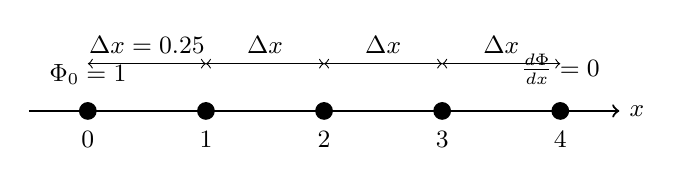
\begin{tikzpicture}[scale=1.5, every node/.style={font=\small}]
        \draw[thick, ->] (-0.5,0) -- (4.5,0) node[right] {$x$};
        \foreach \x/\label in {0/0, 1/1, 2/2, 3/3, 4/4} {
                \filldraw (\x,0) circle (2pt) node[below=4pt] {$\label$};
            }
        \draw[<->] (0,0.4) -- (1,0.4) node[midway,above] {$\Delta x = 0.25$};
        \draw[<->] (1,0.4) -- (2,0.4) node[midway,above] {$\Delta x$};
        \draw[<->] (2,0.4) -- (3,0.4) node[midway,above] {$\Delta x$};
        \draw[<->] (3,0.4) -- (4,0.4) node[midway,above] {$\Delta x$};
        \node[above=6pt] at (0,0) {$\Phi_0=1$};
        \node[above=6pt] at (4,0) {$\frac{d\Phi}{dx}=0$};
    \end{tikzpicture}
    \caption{Representation of the One-Dimensional Finite Difference Grid Discretization}
\end{figure}

Discretizing the domain into 4 equal intervals ($\Delta x = 0.25$, nodes $x_0=0, x_1=0.25, x_2=0.5, x_3=0.75, x_4=1.0$):

At interior nodes $i = 1, 2, 3$:
\begin{equation}
    \Phi_{i+1} - 2\Phi_i + \Phi_{i-1} = 6 x_i \Delta x^2
\end{equation}

\begin{itemize}
    \item \textbf{Node 1 ($x_1 = 0.25$):} $\Phi_2 - 2\Phi_1 + \Phi_0 = 6(0.25)(0.25)^2 = 0.09375$
    \item \textbf{Node 2 ($x_2 = 0.50$):} $\Phi_3 - 2\Phi_2 + \Phi_1 = 6(0.50)(0.25)^2 = 0.18750$
    \item \textbf{Node 3 ($x_3 = 0.75$):} $\Phi_4 - 2\Phi_3 + \Phi_2 = 6(0.75)(0.25)^2 = 0.28125$
\end{itemize}

Boundary equations:
\begin{itemize}
    \item $\Phi_0 = 1 \implies -2\Phi_1 + \Phi_2 = 0.09375 - 1 = -0.90625$ (Dirichlet BC)
    \item $\frac{\Phi_4 - \Phi_3}{\Delta x} = 0 \implies -\Phi_3 + \Phi_4 = 0$ (Neumann BC)
\end{itemize}

System of equations in matrix form $A\mathbf{\Phi} = \mathbf{b}$:
\begin{equation}
    \begin{bmatrix}
        -2 & 1  & 0  & 0 \\
        1  & -2 & 1  & 0 \\
        0  & 1  & -2 & 1 \\
        0  & 0  & -1 & 1
    \end{bmatrix}
    \begin{bmatrix}
        \Phi_1 \\ \Phi_2 \\ \Phi_3 \\ \Phi_4
    \end{bmatrix}
    =
    \begin{bmatrix}
        -0.90625 \\ 0.18750 \\ 0.28125 \\ 0
    \end{bmatrix}
\end{equation}

\textit{Note:} Numerical error is minimized at Dirichlet boundaries because the exact solution value is known, whereas error is larger at Neumann boundaries due to derivative approximation.

\section{Convection-Diffusion Equation \& Stability}

\subsection{Governing Transport Equation}

The 2D momentum transport (Navier-Stokes) equation combines unsteady, convective, and diffusive terms:
\begin{equation}
    \frac{\partial u}{\partial t} + u\frac{\partial u}{\partial x} + v\frac{\partial u}{\partial y} = -\frac{1}{\rho}\frac{\partial P}{\partial x} + g_x + \nu \left( \frac{\partial^2 u}{\partial x^2} + \frac{\partial^2 u}{\partial y^2} \right)
\end{equation}

For a 1D steady convection-diffusion model:
\begin{equation}
    3\frac{d^2\Phi}{dx^2} = 75\frac{d\Phi}{dx} - 8x
\end{equation}

Applying central differences to both terms:
\begin{equation}
    3\left(\frac{\Phi_{i+1} - 2\Phi_i + \Phi_{i-1}}{\Delta x^2}\right) = 75\left(\frac{\Phi_{i+1} - \Phi_{i-1}}{2\Delta x}\right) - 8x_i
\end{equation}

Rearranging into standard form:
\begin{equation}
    \left(\frac{3}{\Delta x^2} - \frac{75}{2\Delta x}\right)\Phi_{i+1} - \frac{6}{\Delta x^2}\Phi_i + \left(\frac{3}{\Delta x^2} + \frac{75}{2\Delta x}\right)\Phi_{i-1} = -8x_i
\end{equation}

\subsection{Peclet Number and Upwinding}

Central differencing for convection can lead to non-physical oscillations when convection dominates over diffusion.

\begin{itemize}
    \item \textbf{Peclet Number:} $Pe = \frac{u \Delta x}{K}$ (where $u$ is velocity and $K$ is diffusivity).
    \item If $Pe < 2$, the central difference scheme is stable.
    \item If $Pe > 2$, an \textbf{upwind scheme} must be selected based on flow direction:
          \begin{itemize}
              \item Flow left to right ($u > 0$): Use backward difference for convection.
              \item Flow right to left ($u < 0$): Use forward difference for convection.
          \end{itemize}
\end{itemize}

\section{2D Finite Difference Method}

\subsection{2D Laplace / Poisson Equation}

\begin{equation}
    \frac{\partial^2\Phi}{\partial x^2} + \frac{\partial^2\Phi}{\partial y^2} = 0
\end{equation}

Assuming equal grid spacing ($\Delta x = \Delta y = \Delta$), the 5-point stencil is:
\begin{equation}
    \frac{1}{\Delta^2} \left( \Phi_{i+1, j} + \Phi_{i-1, j} + \Phi_{i, j+1} + \Phi_{i, j-1} - 4\Phi_{i,j} \right) = 0
\end{equation}

\subsection{Grid Indexing (1D Flattening)}

To convert 2D grid coordinates $(i,j)$ to a 1D global array index for matrix solving:
\begin{equation}
    \mathrm{ID} = j \times N_x + i + 1
\end{equation}

\subsection{Cross-Stream (False) Diffusion}

When grid lines are not aligned with the velocity vector at angle $\theta$, numerical false diffusion occurs:
\begin{equation}
    K_{\text{false}} = \frac{\sqrt{u^2 + v^2} \, \Delta x \, \Delta y \, \sin(2\theta)}{4(\Delta y \sin^3\theta + \Delta x \cos^3\theta)}
\end{equation}
False diffusion reaches its maximum at $\theta = 45^\circ$.

\section{Finite Volume Method (FVM)}

\subsection{Divergence Theorem \& General Conservation Equation}

The Divergence Theorem converts domain integrals into surface flux integrals:
\begin{align}
    \text{1D:} \quad & \int_a^b \frac{d\Phi}{dx} \, dx = \Phi(b) - \Phi(a)                                    \\
    \text{2D:} \quad & \iint_A (\nabla \cdot \vec{u}) \, dA = \oint_{\partial A} \vec{u} \cdot \hat{n} \, dS  \\
    \text{3D:} \quad & \iiint_V (\nabla \cdot \vec{u}) \, dV = \iint_{\partial V} \vec{u} \cdot \hat{n} \, dA
\end{align}

Integrating the steady general conservation equation over a control volume $A$:
\begin{equation}
    \oint_{\partial A} \Phi (\vec{v} \cdot \hat{n}) \, dS = \oint_{\partial A} K (\nabla \Phi \cdot \hat{n}) \, dS + \iint_A Q \, dA
\end{equation}

\subsection{1D Diffusion Equation in FVM}

\begin{figure}[H]
    \centering
    \begin{tikzpicture}[scale=1.5, every node/.style={font=\small}]
        \draw[thick] (0,0) -- (4,0);
        \draw[thick] (0,-0.4) -- (0,0.4) node[above] {$x_l$};
        \draw[thick] (4,-0.4) -- (4,0.4) node[above] {$x_r$};
        \filldraw (2,0) circle (2.5pt) node[below=4pt] {$\Phi_C \, (x_c)$};
        \filldraw (-1.5,0) circle (2pt) node[below=4pt] {$\Phi_W$};
        \filldraw (5.5,0) circle (2pt) node[below=4pt] {$\Phi_E$};
        \draw[dashed] (-1,-0.4) -- (-1,0.4);
        \draw[dashed] (5,-0.4) -- (5,0.4);
        \draw[<->] (0,-0.7) -- (4,-0.7) node[midway,below] {$\Delta x$};
    \end{tikzpicture}
    \caption{Representation of a One-Dimensional Finite Volume Control Cell}
\end{figure}

\begin{equation}
    K \frac{d}{dx}\left(\frac{d\Phi}{dx}\right) = Q(x)
\end{equation}

Integrating over control volume $[x_l, x_r]$:
\begin{equation}
    K \left( \left.\frac{d\Phi}{dx}\right|_{x_r} - \left.\frac{d\Phi}{dx}\right|_{x_l} \right) = Q(x_c) (x_r - x_l)
\end{equation}

Approximating face gradients using central differences between cell centers:
\begin{equation}
    \Phi_{i+1} - 2\Phi_i + \Phi_{i-1} = \frac{Q(x_c)}{K} \Delta x^2
\end{equation}

\subsection{Boundary Conditions in 1D FVM}

Because solutions in FVM are stored at cell centers ($x_c$), boundary conditions require explicit face formulations:

\paragraph{Dirichlet Boundary ($\Phi = \Phi_0$ at left boundary face $x_l$):}
\begin{equation}
    K \left( \frac{\Phi_{i+1} - \Phi_i}{\Delta x} - \frac{\Phi_i - \Phi_0}{\Delta x / 2} \right) = Q(x_c) \Delta x \implies \Phi_{i+1} - 3\Phi_i = \frac{Q(x_c)}{K}\Delta x^2 - 2\Phi_0
\end{equation}

\paragraph{Dirichlet Boundary ($\Phi = \Phi_0$ at right boundary face $x_r$):}
\begin{equation}
    K \left( \frac{\Phi_0 - \Phi_i}{\Delta x / 2} - \frac{\Phi_i - \Phi_{i-1}}{\Delta x} \right) = Q(x_c) \Delta x \implies \Phi_{i-1} - 3\Phi_i = \frac{Q(x_c)}{K}\Delta x^2 - 2\Phi_0
\end{equation}

\paragraph{Neumann Boundary ($\left.\frac{d\Phi}{dx}\right|_{x_l} = \gamma$ at left boundary face $x_l$):}
\begin{equation}
    K \left( \frac{\Phi_{i+1} - \Phi_i}{\Delta x} - \gamma \right) = Q(x_c) \Delta x \implies \Phi_{i+1} - \Phi_i = \frac{Q(x_c)}{K}\Delta x^2 + \gamma \Delta x
\end{equation}

\section{2D Finite Volume Method}

\begin{figure}[H]
    \centering
    \begin{tikzpicture}[scale=1.2, every node/.style={font=\small}]
        \draw[thick] (0,0) rectangle (3,3);
        \filldraw (1.5,1.5) circle (2.5pt) node[above right] {$\Phi_C$};
        \filldraw (1.5,4.2) circle (2pt) node[above] {$\Phi_N$};
        \filldraw (1.5,-1.2) circle (2pt) node[below] {$\Phi_S$};
        \filldraw (4.2,1.5) circle (2pt) node[right] {$\Phi_E$};
        \filldraw (-1.2,1.5) circle (2pt) node[left] {$\Phi_W$};

        \node[above] at (1.5,3) {$n$};
        \node[below] at (1.5,0) {$s$};
        \node[right] at (3,1.5) {$e$};
        \node[left] at (0,1.5) {$w$};

        \draw[<->] (0,-0.4) -- (3,-0.4) node[midway,below] {$\Delta x$};
        \draw[<->] (-0.4,0) -- (-0.4,3) node[midway,left] {$\Delta y$};
    \end{tikzpicture}
    \caption{Representation of Two-Dimensional Finite Volume Cell Centroid and Face Stencil}
\end{figure}

Integrating over a 2D control volume cell with faces East ($e$), West ($w$), North ($n$), South ($s$):
\begin{equation}
    \left(\frac{\partial\Phi}{\partial x}\right)_e \Delta y - \left(\frac{\partial\Phi}{\partial x}\right)_w \Delta y + \left(\frac{\partial\Phi}{\partial y}\right)_n \Delta x - \left(\frac{\partial\Phi}{\partial y}\right)_s \Delta x = \frac{Q(x_c,y_c)}{K} \Delta x \Delta y
\end{equation}

For a square grid ($\Delta x = \Delta y = \Delta$):
\begin{equation}
    \Phi_E + \Phi_W + \Phi_N + \Phi_S - 4\Phi_C = \frac{Q(x_c,y_c)}{K} \Delta^2
\end{equation}

\paragraph{Dirichlet BC on West Face ($\Phi = \Phi_0$):}
\begin{equation}
    \Phi_E + \Phi_N + \Phi_S - 5\Phi_C = \frac{Q(x_c,y_c)}{K} \Delta^2 - 2\Phi_0
\end{equation}

\paragraph{Neumann BC on South Face ($\left.\frac{\partial\Phi}{\partial y}\right|_s = \gamma$):}
\begin{equation}
    \Phi_E + \Phi_W + \Phi_N - 3\Phi_C = \frac{Q(x_c,y_c)}{K} \Delta^2 + \gamma \Delta x
\end{equation}

\section{Time-Dependent Problems (Time Marching)}

\subsection{1D Unsteady Convection-Diffusion Equation}

\begin{equation}
    \frac{\partial\Phi}{\partial t} = -u \frac{\partial\Phi}{\partial x} + K \frac{\partial^2\Phi}{\partial x^2} + Q(x)
\end{equation}

\subsection{Explicit Euler Method}

Applying a forward difference in time and central differences in space:
\begin{equation}
    \frac{\Phi_i^{n+1} - \Phi_i^n}{\Delta t} = -u \left(\frac{\Phi_{i+1}^n - \Phi_{i-1}^n}{2\Delta x}\right) + K \left(\frac{\Phi_{i+1}^n - 2\Phi_i^n + \Phi_{i-1}^n}{\Delta x^2}\right) + Q(x_i)
\end{equation}

Solving explicitly for the state at time level $n+1$:
\begin{equation}
    \Phi_i^{n+1} = \left(-\frac{u\Delta t}{2\Delta x} + \frac{K\Delta t}{\Delta x^2}\right) \Phi_{i+1}^n + \left(1 - \frac{2K\Delta t}{\Delta x^2}\right) \Phi_i^n + \left(\frac{u\Delta t}{2\Delta x} + \frac{K\Delta t}{\Delta x^2}\right) \Phi_{i-1}^n + Q(x_i)\Delta t
\end{equation}

\subsection{Implicit Euler Method}

Applying a backward difference in time, evaluating spatial terms at time level $n+1$:
\begin{equation}
    \left(-\frac{u\Delta t}{2\Delta x} - \frac{K\Delta t}{\Delta x^2}\right) \Phi_{i-1}^{n+1} + \left(1 + \frac{2K\Delta t}{\Delta x^2}\right) \Phi_i^{n+1} + \left(\frac{u\Delta t}{2\Delta x} - \frac{K\Delta t}{\Delta x^2}\right) \Phi_{i+1}^{n+1} = \Phi_i^n + Q(x_i)\Delta t
\end{equation}

Implicit time marching requires matrix inversion at every step but is unconditionally stable regardless of Courant number ($Co = \frac{u \Delta t}{\Delta x}$).

\end{document}
